\documentclass[border=3pt]{standalone}
% Preâmbulo compartilhado pelos diagramas TikZ da aula 5 de IHC (Processos de Design)
\usepackage[T1]{fontenc}
\usepackage[utf8]{inputenc}
\usepackage{lmodern}
\usepackage{amsmath}
\usepackage{xcolor}
\usepackage{tikz}
\usetikzlibrary{arrows.meta,angles,quotes,decorations.pathmorphing,calc,
                positioning,shapes.geometric,shapes.misc,backgrounds,fit,
                math}

% Paleta (mesma dos SVGs originais)
% Paleta da disciplina de IHC: acento roxo (#755099), da capa do livro.
% (o nome "dblue" é mantido para não alterar todos os diagramas)
\definecolor{dblue}{HTML}{755099}
\definecolor{dorange}{HTML}{B3541E}
\definecolor{dgreen}{HTML}{4A7C59}
\definecolor{dred}{HTML}{9C4B4B}
\definecolor{dcream}{HTML}{F4F1EA}
\definecolor{dshade}{HTML}{DDD7C9}

% Função gaussiana (não normalizada por padrão de escala visual)
\pgfmathdeclarefunction{gauss}{3}{%
  \pgfmathparse{1/(#3*sqrt(2*pi))*exp(-((#1-#2)^2)/(2*#3^2))}%
}

% Estilos comuns (prefixo d... para não colidir com chaves internas do pgf)
\tikzset{
  >={Stealth[length=2mm]},
  dguide/.style={gray!55, dashed, line width=0.4pt},
  daxis/.style={gray!60, line width=0.7pt, ->},
  dbody/.style={fill=black!3, draw=black!80, line width=1pt},
  dacc/.style={draw=dblue, line width=1pt},
  dlbl/.style={black!55, font=\small},
  dsub/.style={black!45, font=\footnotesize},
  dstate/.style={circle, draw=black!80, fill=dcream, line width=1pt,
                 minimum size=17mm, font=\large, inner sep=1pt},
  dobs/.style={circle, draw=black!80, fill=dshade, line width=1pt,
               minimum size=14mm, font=\large, inner sep=1pt},
  dbox/.style={rounded corners=2pt, draw=black!80, fill=dcream, line width=1pt,
               align=center, inner sep=6pt},
  dop/.style={circle, draw=black!80, fill=white, line width=1pt,
              minimum size=6mm, inner sep=0pt, font=\small},
  dtrans/.style={->, dblue, line width=1pt},
  dmeas/.style={->, dorange, line width=1pt},
  dcurve/.style={line width=1pt, dblue},
  dcurveb/.style={line width=1.4pt, dorange},
}

\begin{document}
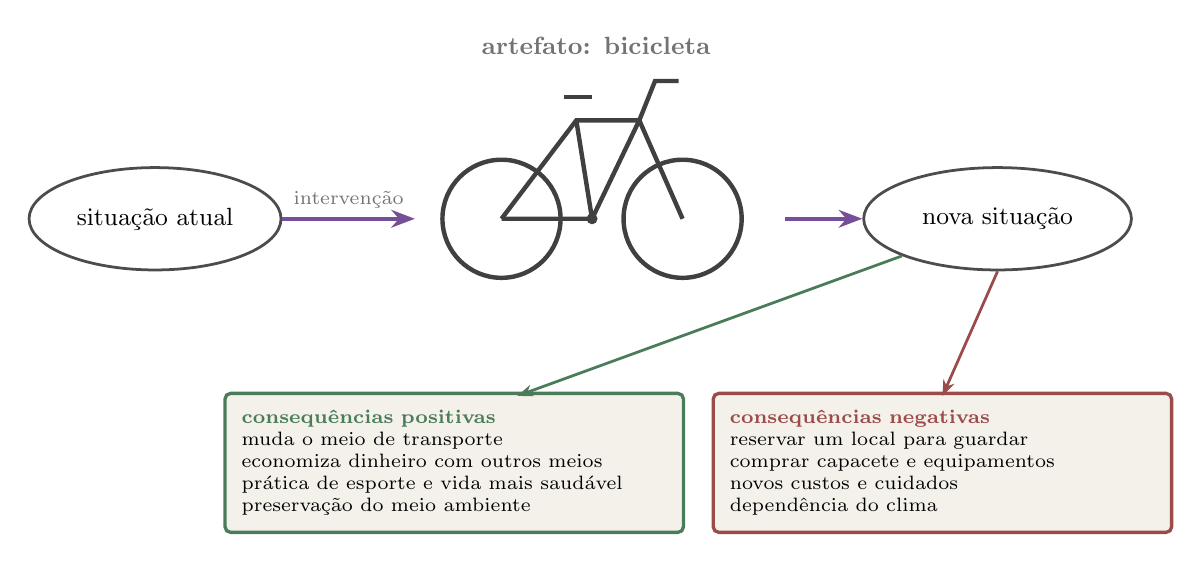
\begin{tikzpicture}[x=1cm,y=1cm]

  % bicicleta
  \begin{scope}[shift={(5.0,2.0)}, line width=1.6pt, draw=black!75]
    \draw (0,0) circle (0.75); \draw (2.3,0) circle (0.75);
    \draw (0,0) -- (0.95,1.25) -- (1.75,1.25) -- (2.3,0);
    \draw (0.95,1.25) -- (1.15,0) -- (0,0);
    \draw (1.15,0) -- (1.75,1.25);
    \draw (0.8,1.55) -- (1.15,1.55) ;
    \draw (1.75,1.25) -- (1.95,1.75) -- (2.25,1.75);
    \fill[black!75] (1.15,0) circle (0.07);
  \end{scope}
  \node[dlbl, font=\small\bfseries] at (6.2,4.2) {artefato: bicicleta};

  \node[ellipse, draw=black!70, fill=white, line width=1pt, minimum width=3.2cm, minimum height=1.3cm, font=\small] (s1) at (0.6,2.0) {situação atual};
  \draw[dtrans, line width=1.6pt, -{Stealth[length=3mm]}] (s1.east) -- (3.9,2.0) node[midway, above, dlbl, font=\scriptsize] {intervenção};

  \node[ellipse, draw=black!70, fill=white, line width=1pt, minimum width=3.4cm, minimum height=1.3cm, font=\small] (s2) at (11.3,2.0) {nova situação};
  \draw[dtrans, line width=1.6pt, -{Stealth[length=3mm]}] (8.6,2.0) -- (s2.west);

  \node[dbox, draw=dgreen, line width=1.2pt, text width=5.4cm, align=left, font=\scriptsize] at (4.4,-1.1) {\textbf{\textcolor{dgreen}{consequências positivas}}\\ muda o meio de transporte\\ economiza dinheiro com outros meios\\ prática de esporte e vida mais saudável\\ preservação do meio ambiente};
  \node[dbox, draw=dred, line width=1.2pt, text width=5.4cm, align=left, font=\scriptsize] at (10.6,-1.1) {\textbf{\textcolor{dred}{consequências negativas}}\\ reservar um local para guardar\\ comprar capacete e equipamentos\\ novos custos e cuidados\\ dependência do clima};
  \draw[dtrans, dgreen] (s2.south west) -- (5.2,-0.25);
  \draw[dtrans, dred] (s2.south) -- (10.6,-0.25);

\end{tikzpicture}
\end{document}
